\clearpage
\subsection{Assignment Statement (with Arrays)} % (fold)
\label{sub:assignment_statement_with_arrays_}

The assignment statement allows you to store a value in a variable. This can now be extended to allow you to store a value in an element of an array. To achieve this you indicate the array you want to store the value in, as well as the index at which the value is to be stored.

\begin{figure}[h]
   \centering
   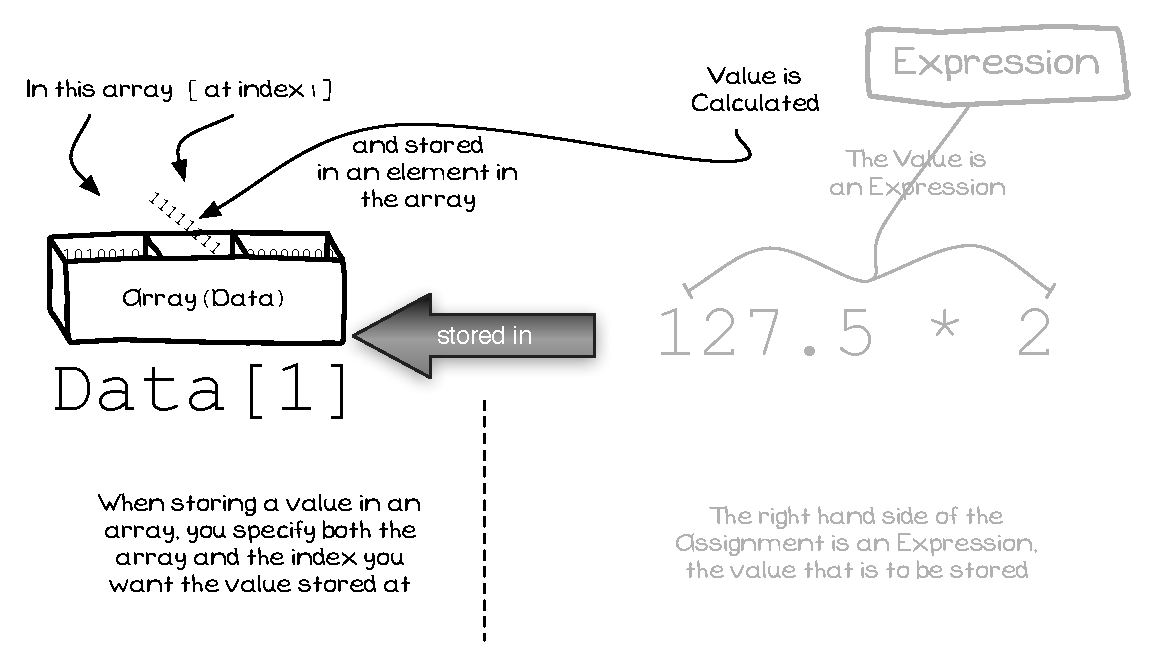
\includegraphics[width=\textwidth]{./topics/arrays/diagrams/AssignmentWithArray} 
   \caption{Arrays allow you to store multiple values in a variable}
   \label{fig:assignment-with-arrays}
\end{figure}

\mynote{
\begin{itemize}
  \item The assignment statement is an \textbf{action}, storing a value in a variable or array.
  \item When working with arrays you specify the array, and index at which to store the value.
  \item This stores a value into an element of an array.
  \item The two snippets below indicate how this is coded in C and Pascal. In each case \texttt{data} is the name of the array variable, and 1 is the index of the second element. The code in the snippet stores a 255 in the second element of the array.
\end{itemize}
}


\csection{In C you can achieve this using: \csnipet{data[1] =  127.5 * 2;}. }

\passection{In Pascal you can achieve this using: \passnipet{data[1] :=  127.5 * 2;}.}

\clearpage
\subsubsection{Assigning all elements of an array} % (fold)
\label{ssub:assigning_all_elements_of_an_array}

Many languages also allow you to copy the entire contents of an array into another array. In these cases each of the elements of one array are copied into the elements of the destination array (left hand side of the assignment).

\begin{figure}[h]
   \centering
   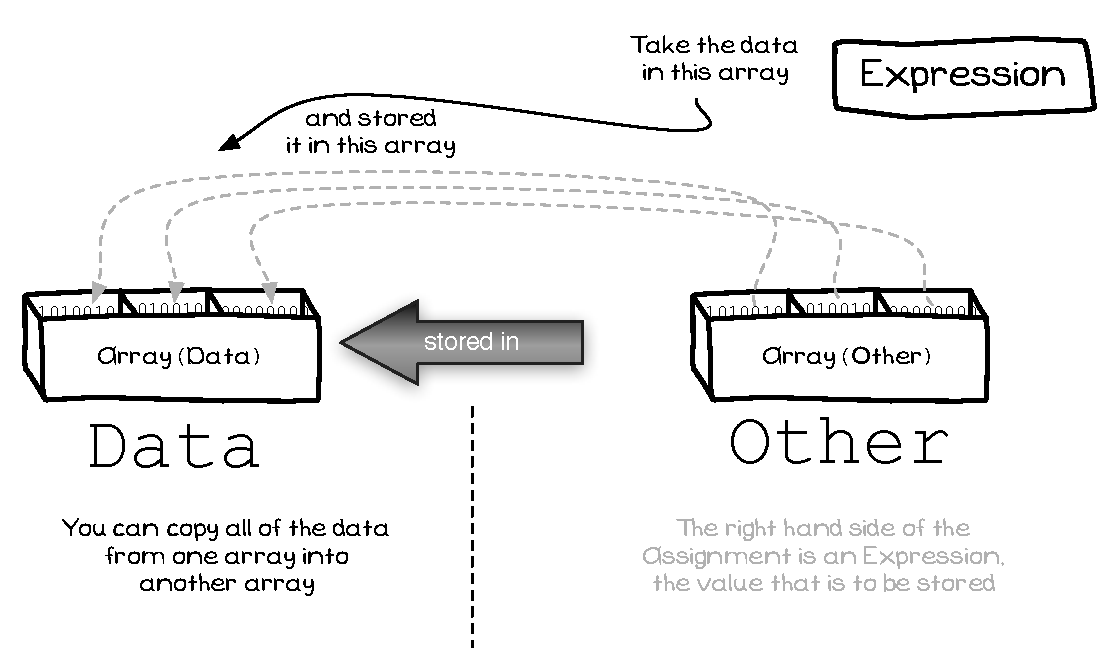
\includegraphics[width=\textwidth]{./topics/arrays/diagrams/AssignmentWithArray2} 
 \caption{All of the elements of an array can be copied across in the assignment statement}
 \label{fig:assignment-with-arrays2}
\end{figure}

\mynote{
\begin{itemize}
  \item The size of the two arrays should match.
  \item The value from each of the elements of the array on the right hand side will be copied into the matching element in the array on the left hand side.
\end{itemize}
}

\csection{This \textbf{cannot} be done in C with an assignment statement, rather it is achieved using the \texttt{memcopy} function. The code for this is as follows, with \texttt{sz} being the number of elements to copy. \csnipet{memcpy(data, source, size_of(double) * sz)}}

\passection{In Pascal you can achieve this using: \passnipet{data := other;}.}

% subsubsection assigning_all_elements_of_an_array (end)

% subsection assignment_statement_with_arrays_ (end)